\documentclass[12pt,a4paper]{article}
\usepackage[utf8]{inputenc}
\usepackage{a4wide}
\usepackage[spanish,es-tabla]{babel}
\usepackage[spanish]{babel}
\usepackage{amsmath}
\usepackage{amsthm}
\usepackage{booktabs}
\usepackage{multirow} 
\usepackage{placeins}
\usepackage{hyperref}
\usepackage{fancyhdr}
\usepackage{titling}
\usepackage[T1]{fontenc}
\usepackage{graphicx}
\usepackage{floatrow}
\usepackage{siunitx}
\usepackage{listings}
\usepackage{minted}
\usepackage[table,xcdraw]{xcolor}
\usepackage{subcaption}
\usepackage{ragged2e}
\setminted[C]{fontsize=\footnotesize, tabsize=4}
\setminted[make]{fontsize=\footnotesize, tabsize=4}
\setminted[gas]{fontsize=\footnotesize, tabsize=2}
\setminted[bash]{fontsize=\footnotesize, tabsize=4}


\graphicspath{{images/}}

\newfloatcommand{capbtabbox}{table}[][\FBwidth]
\newcommand{\rulesep}{\unskip\ \vrule\ }

\sisetup{
locale=DE,
per-mode=fraction,
separate-uncertainty,
% exponent-to-prefix,
% prefixes-as-symbols=false,
list-units=brackets,
range-units=brackets,
multi-part-units=brackets,
table-unit-alignment=left,
% load=prefixed,
load-configurations=abbreviations,
}

\newcommand{\thetitle}{Trabajo Práctico 2: Machine Learning}
\newcommand{\theauthor}{Pérez Andrade Violeta\\Sinisi Fernando}
\newcommand{\thedate}{Segundo Cuatrimestre de 2020}

\hypersetup{
    unicode=false,
    pdftoolbar=true,
    pdfmenubar=true,
    pdffitwindow=false,
    pdftitle={\thetitle},
    pdfsubject={},
    pdfkeywords={6620-Organización de Datos},
    colorlinks=true,
    linkcolor=black,
    citecolor=black,
    filecolor=magenta,
    urlcolor=cyan
}

%%%%%%%%%%%%%%%%%%%%%%%%%%%%%%%%%%%%%%%%%%%%%%%%%%%%%%%%%%


\pagestyle{fancy}
\fancyhf{}
\lhead{Trabajo Práctico 2}
\rhead{Organización de Datos}
\cfoot{\thepage}

\setlength{\headheight}{14.5pt}


\begin{document}


\begin{titlepage}
	\centering
    \vspace*{2.5cm}

    
\includegraphics[scale = 0.7]{imgs/logofiuba.jpg}\\[2.0 cm]

	\textsc{\Large 75.06 Organización de Datos}\\[0.7 cm]
	\textsc{Facultad de Ingeniería, Universidad de Buenos Aires}\\[0.5 cm]

	\rule{0.94\linewidth}{0.2 mm} \\[0.4 cm]
	{\huge \bfseries \thetitle}\\
	\rule{0.94\linewidth}{0.2 mm} \\[1.2 cm]

    \begin{tabular}{lll} % Datos del alumno
        \toprule
        Padrón & Alumno & Dirección de correo \\
        \midrule
        101456 & Pérez Andrade, Violeta  & viperez@fi.uba.ar \\
        99139 & Sinisi, Fernando & fsinisi@fi.uba.ar \\
        \bottomrule
    \end{tabular}\\


    \vspace*{1cm}

\end{titlepage}

\tableofcontents
\newpage

\section{Introducción}

El objetivo principal del trabajo práctico es construir un modelo capaz de estimar la probabilidad de éxito para cada oportunidad de negocio de la empresa frío-frío, con el menor error posible. El error de la solución (inversamente: su calidad) es calculado con la ecuación de log-likelihood:
\begin{equation}
\operatorname{loss}(\mathbf{y}, \hat{\mathbf{y}})=-\frac{1}{N} \sum_{i=1}^{N} y_{i} \log \left(\hat{y}_{i}\right)+\left(1-y_{i}\right) \log \left(1-\hat{y}_{i}\right)
\end{equation}
siendo \textit{y} un vector binario con el éxito real de cada oportunidad y \textit{ŷ} un vector con las probabilidades continuas. \\
Este modelo, se realizo con algoritmos de Machine Learning, lo cual busca poder generar clasificaciones en base a un entrenamiento sobre información pasada, las cuales luego son validadas. En el presente trabajo se probaron distintos algoritmos, los cuales hacen uso de los datos en distinta manera. Por esto ultimo es muy importante saber cuales datos usar y como codificarlos. \\
De esta forma, fueron brindados dos sets de datos: 
\textit{Train\_TP2\_Datos\_2020-2C.csv} y \textit{Test\_TP2\_Datos\_2020-2C.csv} los cuales fueron utilizados, respectivamente, para entrenar los modelos, y luego realizar las predicciones. \\
En ambos sets de datos, cada fila representa un ítem
vendido para una ’oportunidad’ la cual consiste en un proyecto de venta o instalación de equipos para un cliente. La venta se estructura alrededor de TRF (Toneladas de refrigeración) y puede ser una oportunidad que resultó exitosa o no. \\
El código correspondiente se puede hallar en el siguiente repositorio: \url{https://github.com/FernandoSinisi/Orga-Datos-2C-2020}
\newpage
  

\section{Limpieza de datos}
La limpieza de los datos es un proceso fundamental para identificar datos aberrantes, faltantes o atípicos. Para el caso del set de datos utilizado en este trabajo, en el primer trabajo practico notamos que había ciertas columnas cuyo contenido era nulo en mas del 60\% de su totalidad. Las mismas son:
\begin{itemize}
    \item Last\_Activity
    \item Actual\_Delivery\_Date
    \item Price
    \item Size
    \item Product\_Type
    \item Brand
    \item Product\_Category\_B
    \item Source 
\end{itemize}
Por otra parte, la columna Sales\_Contract\_No no se utilizo dado que se advirtió que la misma contenía un leak del target. \\
Una vez eliminadas estas columnas, quedaron algunos datos vacíos pero no en gran cantidad, por lo que, para ciertos algoritmos que no podían entrenar/predecir con datos faltantes, se opto por reemplazar los mismos con 0.

\section{Feature Engineering}
Se buscaron todos los atributos o relaciones posibles de las variables contenidas en el set de
datos proporcionado para el trabajo para luego realizar una selección de features y poder utilizar los mas relevantes para los algoritmos a aplicar.\\
De esta forma, a partir de los features ya existentes se agregaron lo siguientes:
\begin{itemize}
    \item Diferencia en días: Indica la diferencia, en días, entre la fecha de creación de la oportunidad y la ultima modificación de la misma.
    \item A partir de los features de tipo fecha:
    \begin{itemize}
        \item Planned\_Delivery\_End\_Date
        \item Planned\_Delivery\_Start\_Date
        \item Quote\_Expiry\_Date
        \item Opportunity\_Created\_Date
        \item Last\_Modified\_Date
    \end{itemize}
    para cada uno, se crearon dos columnas: DOY y Year las cuales representan, respectivamente, el día de año y el año de la fecha.
    \item También a partir de variables categóricos creamos algunos features que sean la concatenación de estas variables como:
    \begin{itemize}
        \item Delivery\_Quarter\_of\_Year
        \item Region\_Territory\_Country
        \item Product\_Family\_Name
    \end{itemize}
    \item Por otro lado creamos columnas binarias en base a otros features ya existentes:
    \begin{itemize}
        \item ASP\_Higher\_Mean: con valor 1 si el ASP es mayor al promedio, 0 de lo contrario.
        \item TRF\_Higher\_Mean: con valor 1 si las TRF son mayores al promedio, 0 de lo contrario.
        \item Same\_Owner: con valor 1 si el responsable de la cuenta cliente es el mismo que el responsable de la oportunidad, 0 de lo contrario. 
        \item Last\_Modified\_By\_Account\_Owner: con valor 1 si el responsable de la cuenta cliente es el último que modifico la  oportunidad, 0 de lo contrario.
        \item Last\_Modified\_By\_Opportunity\_Owner: con valor 1 si el responsable de la oportunidad  es el último que modifico la  misma, 0 de lo contrario.
    \end{itemize}
\end{itemize}
\subsection{Feature Selection}
Luego de agregar features a los ya existentes con el fin de mejorar las predicciones, encaramos la selección de los mismos para cada modelo de 3 maneras distintas. 
 \begin{itemize}
        \item Usando todos los features: De esta manera entrenaríamos con la mayor cantidad de features, así no privábamos a ningún modelo de alguno de ellos, pero teniendo en cuenta que los distintos modelos pueden no ser tan buenos con muchos features o inclusive tardar muchas horas en entrenarse.
        \item Usando los features mas importantes según xgb: Se realizó una selección usando XgbClassifier entrenando con todas las columnas y obteniendo la importancia de las mismas.
        \begin{center}
            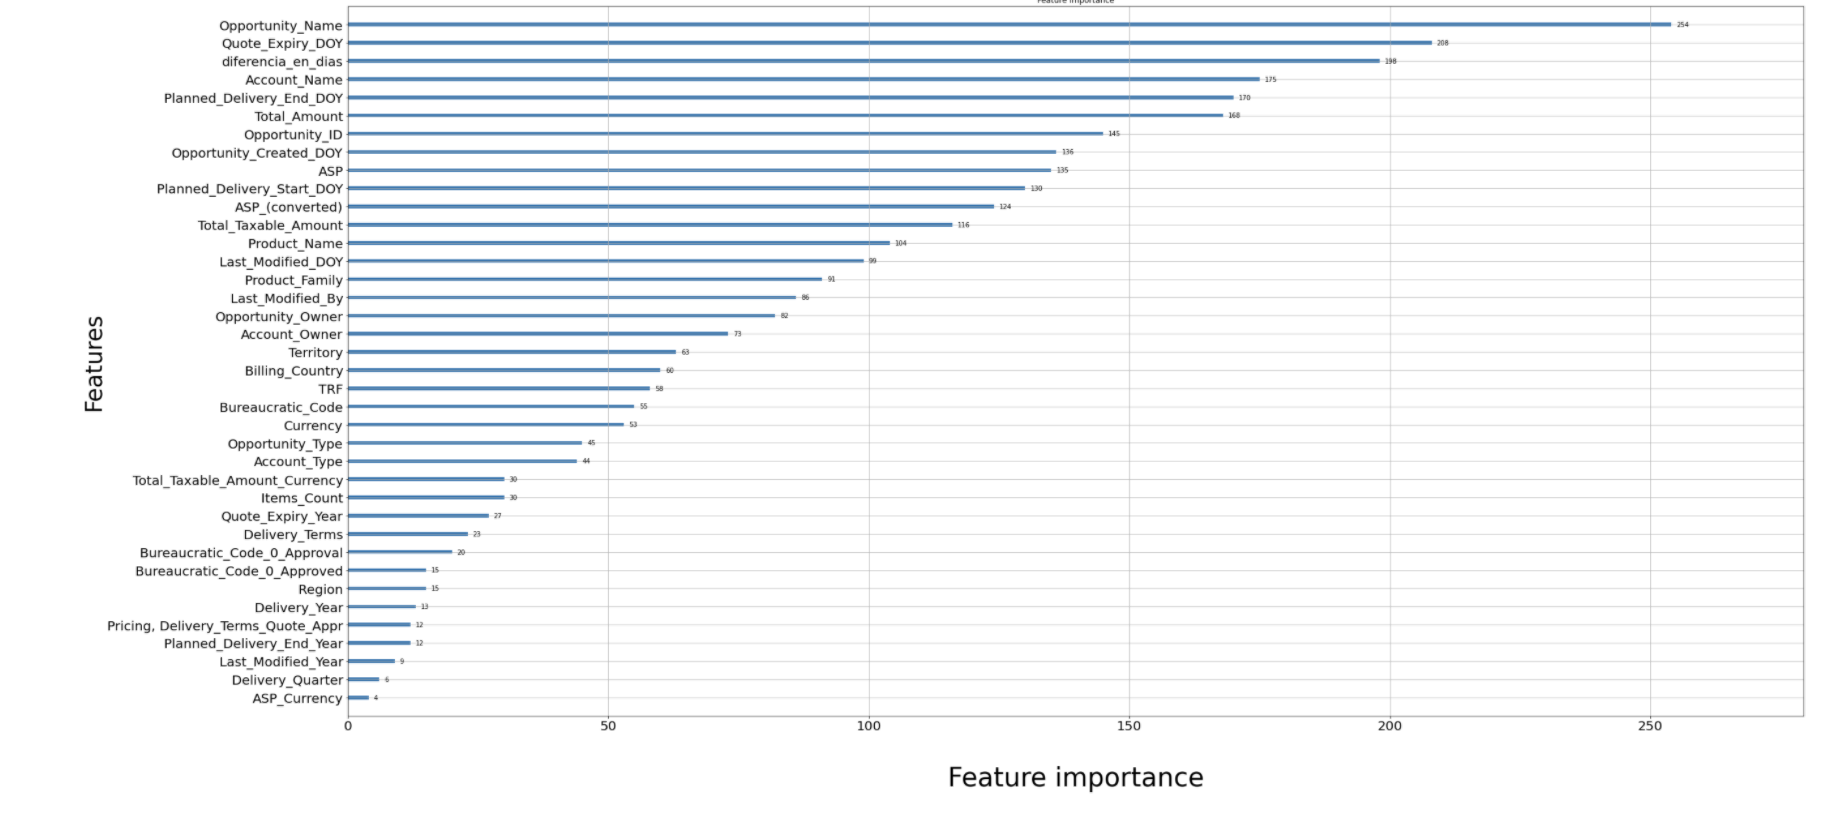
\includegraphics[scale=0.5]{imgs/feature-selection-xgb.png}
        \end{center}
        \item Usando los features mas importante según cada modelo: Con cada modelo se entrenó con todas las columnas y luego a ese modelo se le extrajeron los mejores features y con ellos luego se volvería a entrenar.
        Esto fue útil en los casos donde los encoding usados nos generaron miles de columnas/features donde muchos no aportaban nada al modelo.
    \end{itemize}
    
Como parte del feature selection notamos que ciertos features como \textit{'Opportunity\_Name'} o \textit{'ID'} se consideraban importantes pero en realidad al ser únicas por ítem o por oportunidad lo que ocurría es que algunos modelos los utilizaba incorrectamente por lo que para algunos casos procedimos a eliminarlos.
El caso del \textit{'Opportunity\_ID'} fue un caso particular en el que no podíamos eliminar la columna ya que se necesitaba para poder agrupar los items y también se usaba para generar el submit.

\section{Feature Encoding}
Después del análisis del primer trabajo practico, se evidenció que el set de datos consiste de variables de tipo numéricas, las cuales no necesitan ningún tipo de codificación, y por otra parte variables categóricas. Como no hay ninguna variable de tipo \textbf{string}, se investigo cual era la mejor forma de tratar este tipo de variables(categóricas), y para ello, se utilizaron los encodings que se detallan a continuación:

\subsection{Mean encoding}
\subsection{Binary Encoding}
\subsection{Count Encoder}
Este encoder, también conocido como frequency encoder, tal como su nombre lo indica, trabaja con la frecuencia de cada valor. Es decir, para la columna categórica primero calcula la frecuencia de cata categoría en la columna. Una vez hecho esto, cada valor categórico es reemplazado por la cantidad de veces que este valor aparece en el dataset, previamente calculado.

\subsection{Generalized Linear Mixed Model Encoder Encoder}

El modelo lineal generalizado es una generalización de la regresión lineal. La misma, predice el valor esperado de una cantidad desconocida dada como una combinación lineal de un conjunto de valores observados. Lo cual es útil cuando la variable de respuesta tiene una distribución normal, en cambio, el modelo generalizado sirve también para respuestas con distribución normal, binomial, Poisson y gamma, entre otras. \newline

Este encoder, utiliza el modelo mixto lineal generalizado(GLMM), el cual es una extensión del modelo lineal generalizado el cual incluye efectos aleatorios en el predictor lineal, lo que proporciona un modelo de probabilidad explícito que explica el origen de las correlaciones.\newline

El mismo, no tiene hiperparámetros para tunear. Cuantas menos observaciones tenga una categoría y/o más varíe el resultado para una categoría, mayor será la regularización hacia la media. Este encoding es muy poderoso y puede ser utilizable tanto para targets continuos como binomiales. En al caso de targets binomiales(como en este trabajo), el codificador devuelve probabilidades logarítmicas regularizadas por categoría.

\subsection{Helmert Encoder}

Este encoding pertenece al grupo de los 'Contrast Encoders', explicado en polynomial encoder.
En particular, Helmert, siendo cada "nivel", cada categoría: la media de la variable dependiente para un nivel se compara con la media de la variable dependiente sobre todos los niveles anteriores.

\subsection{JamesStein Encoder}
El estimador de James-Stein devuelve un promedio ponderado de:
\begin{itemize}
    \item La media del target para el valor de la columna 
    \item La media del target, independientemente del valor de la columna
\end{itemize}
James-Stein Encoder reduce el promedio hacia el promedio general. Es un codificador basado en mean encoding. Sin embargo, el mismo tiene una limitación práctica: se definió solo para distribuciones normales.
\subsection{Leave One Out Encoder}

Este encoder es prácticamente igual a mean encoding. La diferencia es que este, excluye el target de la fila actual al calcular la media del target de un nivel para reducir el efecto de valores atípicos. \newline
Por otra parte, se puede agregar algo de ruido a los datos para evitar el overfitting. 

\subsection{MEstimate Encoder}
Este encoding esta basado en mean encoding pero nos da la posibilidad de aplicar smoothing (regularización) para no filtrar tanto el target al set de entrenamiento. En lugar de usar solo el promedio se puede regularizar mediante la siguiente formula:
\begin{center}
    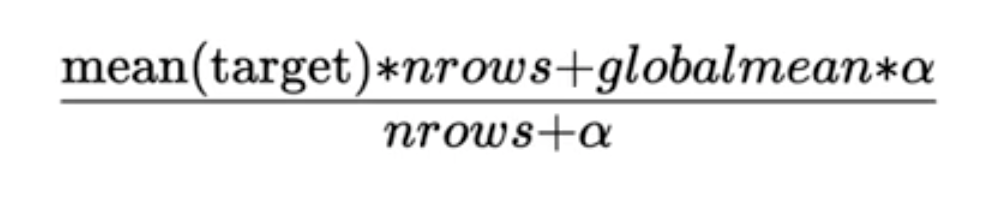
\includegraphics[scale=0.5]{imgs/formula-smoothing.png}
\end{center}
Donde alfa es la variable de regularización que elegimos para nuestro estimador. Como podemos observar si alfa=0 entonces nos queda el promedio del target y es mean-encoding.
\url{https://contrib.scikit-learn.org/category_encoders/mestimate.html}

\subsection{Ordinal Encoder}
Esta codificación es la mas simple de todas y una de las que peor resultado genera. Consiste en que a cada valor de la variable categórica se lo reemplaza por un número asociado a ese valor. Por ej si tengo 4 posibles valores para una variable se asignarían los números 1, 2, 3 y 4.
Esto nos convierte directamente una columna categórica a numérica, pero al usar estos números en los modelos se pueden generar relaciones 'muy extrañas' como que una variable categórica mas otra variable categórica dan una tercera variable categórica. Esto no solo no aportará nada al modelo sino que dará malos resultados.
\url{https://contrib.scikit-learn.org/category_encoders/ordinal.html}

\subsection{WOE Encoder}
El Weight of Evidence encoding codifica las variables categóricas en base a su peso respecto del target mediante la siguiente formula:
\begin{center}
    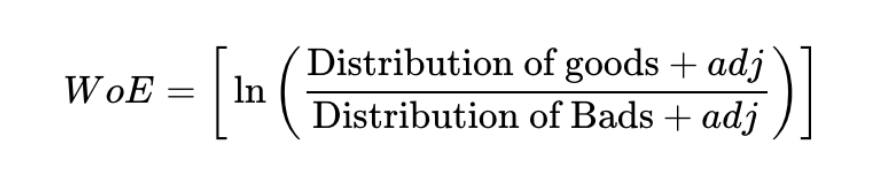
\includegraphics[scale=0.5]{imgs/WOE.png}
\end{center}
donde adj es el factor que evita una división por 0.
Este encoding funciona bien con el modelo de LogisticRegression por utilizar la misma escala logaritmica pero tiene la desventaja de que puede sobreajustar o inclusive tenes distintos valores de una variable categórica con el mismo encoding. 
\url{https://contrib.scikit-learn.org/category_encoders/woe.html}

\subsection{One Hot Encoder}
Este tipo de encoding se basa en que para cada valor categórico de una columna del dataset creara una nueva columna de valor binario, si la row tenía ese valor colocara un 1 en la columna y 0 en las demás. Este encoding podía ser util para features con pocos valores posibles, por lo tanto tendríamos la columna original y tantas columnas nuevas como valores posibles. El punto débil de este encoding es que casos de variables con muchos valores posibles o en el caso de tener muchos features categóricos se necesitaría mucha memoria para entrenar.
\url{https://contrib.scikit-learn.org/category_encoders/onehot.html}

\subsection{Catboost Encoder}
Esta codificación esta basada en Mean Encoding pero se diferencia que calcula la probabilidad en tiempo real, es decir sobre la marcha por lo tanto el dataset no puede estar ordenado por la variable Target. La ventaja de calcularlo sobre la marcha es que para un mismo valor de la variable categórica no se van a obtener los mismos valores y por lo tanto no hay que agregar ruido. Como desventaja al igual que Mean Encoding estoy 'filtrando' el Target por lo tanto hay que tener cuidado con no generar overfitting.
\url{https://contrib.scikit-learn.org/category_encoders/catboost.html}

\subsection{Base N Encoder}
Esta codificación vendría a ser la generalizacion de one-hot-encoding o binary-encoding, es decir elegimos en que base codificar y generará log en base n de la cantidad de valores posibles de la variable a encodear columnas. En otras palabras si elegimos base = 1 entonces sería como one-hot-encoding y si elegimos base = 2 sería como binary-encoding.
\url{https://contrib.scikit-learn.org/category_encoders/basen.html}

\subsection{Sum Encoder}
Es un tipo de encoding también conocido como Effect Encoding o Deviation Encoding, esta basado en one-hot-encoding con la diferencia que en lugar de tener N columnas (1 por cada uno de los N valores posibles de la variable) nos genera N-1 columnas nuevas ya que un valor de la variable se codifica con todos valores -1.
\url{https://contrib.scikit-learn.org/category_encoders/sum.html#category_encoders.sum_coding.SumEncoder}

\subsection{Polynomial Encoder}
Es un encoding perteneciente al grupo de los 'Contrast Encoders' que permiten centran las variables categóricas de manera que la intersección de un modelo no sea el promedio de una categoría, sino la media de todos los puntos de datos en el conjunto de datos.
En este caso este el encoder codifica las variables mediante polinomios. 
\url{https://contrib.scikit-learn.org/category_encoders/polynomial.html}
\newpage
\section{Modelos}
\subsubsection{KNN}
Este algoritmo consiste en encontrar los vecinos más cercanos al punto que se busca clasificar, para luego predecir la clase del punto en cuestión que se obtendrá a partir de la clase mayoritaria presente en sus vecinos.
Los hiperparámetros comunes en KNN son:
\begin{itemize}
    \item n-neighbors: Radio del círculo para la clasificación de los puntos.
    
    \item weights: Puede seleccionarse entre \textit{uniform}, donde cada vecino dentro del perímetro tiene el mismo peso o "distancia", donde los puntos mas cercanos tendrán un mayor peso.
    
    \item metric: Define la metrica para calcular las distancias entre los puntos.
    
\end{itemize}
KNN es uno de los algoritmos mas sencillos de Machine Learning pero definiendo correctamente sus hiperparámetros puede ser muy eficiente. Una desventaja es que se trata de un algoritmo de orden cuadrático por lo que puede tener un gran impacto a la hora de la ejecución.

\subsection{Algoritmos de clasificacion}

\subsubsection{Random Forest}
Este es uno de los algoritmos mas populares para clasificación, el cual crea un conjunto de árboles de decisión a partir de un subconjunto del set de datos de entrenamiento seleccionado al azar. 
Luego, para decidir la clase final del objeto puede utilizar dos formas de decisión, por mayoría de votos o por peso (donde los árboles con alta tasa de error reciben un valor de bajo peso y viceversa, permitiendo que los árboles con baja tasa de error tengan mayor impacto).
Los hiperparámetros comunes en RandomForest son:

\begin{itemize}
    \item n-estimators: Número de árboles.
    
    \item max-features: Cantidad de features a considerar en cada partición del árbol.
    
    \item max-depth: Profundidad de cada árbol.
    
    \item min-samples-split: Cantidad mínima de muestras requeridas para realizar una partición del árbol.
    
    \item min-samples-leaf: Cantidad minima de muestras por cada hoja del arbol
    
    \item bootstrap: Método de selección de muestras para el entrenamiento de cada árbol.
    
\end{itemize}

\subsubsection{SVC}
El objetivo de SVC, es entrenar el set de datos encontrando el mejor hiper-plano que divide a los mismos en categorías.

\subsubsection{NuSVC}
Este algoritmo es similar a SVC (Support Vector Classifier), con la diferencia de que usa como parámetro "nu" el cual controla el número de vectores soportados.

\subsubsection{Naive Bayes Classifier}
Este algoritmo considera cada feature de forma independiente, calculando la probabilidad de que el feature pertenezca a cada una de las categorías, dando como resultado la que contenga el mayor valor de probabilidad. El modelo utilizado para calcular dicha probabilidad esta basado en el teorema de Bayes. Se parte de la suposición de que todos los predictores tienen el mismo efecto en el resultado. Existen diferentes tipos de clasificadores que siguen este modelo.

Los hiperparámetros comunes en Naive Bayes son:
\begin{itemize}
    \item alfa: Parámetro utilizado para realizar el suavizado de Laplace, el cual permite no tener probabilidades nulas a la hora de calcular la probabilidad de que el vector de palabras para un documento se encuentre en alguna de las categorias. Permitiendo siempre generar alguna clasificación. 
\end{itemize}

\subsubsection{XGBoost}
Este algoritmo, es un boosting de arboles de decisión en el cual, cada árbol intenta corregir lo que el anterior no pudo predecir correctamente. A partir de la combinación de varios árboles de decisión, logra buenas predicciones. Boosting es una técnica que funciona según el principio de ensamble. Combina un set de modelos débiles y mejora la precisión de la predicción.\\
Tiene una función objetivo que depende de los parámetros que tiene que aprender. La parte de la predicción esta dada por la diferencia entre el valor de la predicción y el valor real. La predicción final de un boosting es la sumatoria de las predicciones de varios arboles. Una de las cosas que hace que este algoritmo sea tan rápido es que únicamente recibe valores numéricos.
 
Los hiperparametros mas importantes son:
 \begin{itemize}
    \item n-estimators: Número de árboles.
    
    \item learning\_rate: Parametro de contracción. Escala los pesos agregados por un factor n  después de cada paso del árbol, reduce la influencia de cada árbol individual y deja espacio para que los  árboles futuros mejoren el modelo. Tambien sirve para evitar el overfitting.
    
    \item max-depth: Profundidad de cada árbol.
    
    \item objective: La función objetivo, se puede usar alguna de las ya disponibles(como por ejemplo 'binary:logistic', 'reg:linear', 'multi:softprob') o se le puede pasar una función propia.
    
    \item booster: Para seleccionar que booster usar, puede ser: gbtree, gblinear o dart.
    
\end{itemize}

\subsubsection{Red Neuronal}
Este algoritmo no lineal genera las predicciones a partir de la definición de una función de activación. Usualmente las funciones de activación mas comunes suelen ser: \textit{sigmoid}, \textit{relu} o \textit{softmax}. La combinación de distintas funciones de activación es lo que genera la red, donde se cuenta con una capa visible en la cual se reciben los inputs y distintas capas ocultas donde se procesa la información para obtener el output.

\begin{center}
    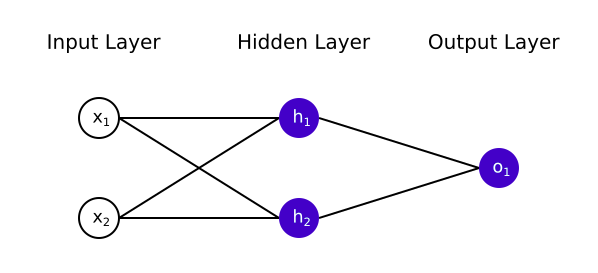
\includegraphics[scale=0.5]{imgs/red neuronal.png}
\end{center}

El objetivo de este algoritmo es el de disminuir el error cuadrático medio (\textit{loss}) para obtener mejores predicciones.
En particular, las redes utilizadas para el procesamiento de lenguaje natural son las Redes Neuronales Recurrentes las cuales, contienen loops en ellas para lograr la persistencia de la información. 

\begin{center}
    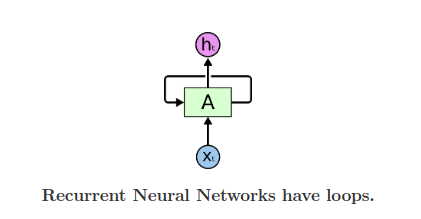
\includegraphics[scale=0.5]{imgs/red neuronal recurrente.png}
\end{center}

\subsubsection{LightGBM}
Este modelo es un algoritmo de \textit{gradient boosting} sobre arboles de decisión.
Produce el modelo predictivo a partir de un conjunto de modelos de predicción débiles. Construye el modelo de forma escalonada y lo generaliza disminuyendo la función de error creciendo verticalmente eligiendo la hoja con mayor "delta loss" para crecer. El crecimiento por hojas, en vez de por niveles, permite reducir aún más el \textit{loss}.

\begin{center}
    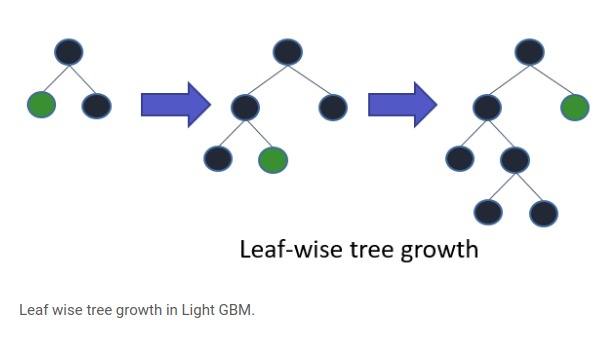
\includegraphics[scale=0.5]{imgs/lightgbm.jpeg}
\end{center}

\subsubsection{Logistic Regression}
Este modelo, es el método de referencia para problemas de clasificación binaria (aquellos donde solo existen dos valores de clase). El mismo, utiliza de base \textit{la función logística} o también llamada \textit{función sigmoidea}, la cual es representada como una curva en forma de S que puede tomar cualquier número real y asignarlo a un valor entre 0 y 1, pero nunca exactamente en esos límites. Logistic Regression predice la probabilidad de que un dato pertenezca a una clase (clase default) y luego esta predicción es transformada a un valor binario con la función logística. 
\section{Ensambles}
\section{Resultados Obtenidos}
\section{Conclusiones}
\end{document}
